\documentclass{beamer}
\usepackage{minted}
\usepackage{epigraph}
\usepackage{subfig}
\usepackage{pgfplots}
\usepackage{tikz}
\usepackage{color, colortbl}

\usetheme{focus}

\definecolor{orangered}{rgb}{1,0.45, 0}

\title{Shor's Algorithm}
\subtitle{Quantum Computer Programming}
\author{Davide Carnemolla}
\titlegraphic{
\includegraphics[scale=0.13]{images/logo.pdf}}
\institute{Department of Mathematics and \\ Computer Science \\ \\ University of Catania}
\date{2022/2023}

\begin{document}
    \begin{frame}
        \maketitle
    \end{frame}
    
    \section{Integer Factorization}

    \begin{frame}{The problem}
        \centering
        
\includegraphics[height=2cm,keepaspectratio]{images/problem.pdf}
        \vspace{0.5cm}
        \begin{block}{Definition}
            Given an integer $N$, the goal of the \textit{integer factorization problem} is to find $k$ primes $p_1^{e_1},p_2^{e_2},\dots,p_k^{e_k}$ such that $N = p_1^{e_1}p_2^{e_2} \dots p_k^{e_k}$ with $e_i \geq 1 \quad \forall i \in \{1, \dots, k\}$.
        \end{block}
        \begin{exampleblock}{Example}
            Given $N = 143$ we know that the solution is the pair $(13, 11).$
        \end{exampleblock}
        
    \end{frame}

    \begin{frame}{RSA}
        \centering
        \begin{block}{RSA}
            $(pk,sk) \leftarrow$ \textbf{keygen}(): \hspace{0.05cm} given two primes $p$ and $q$ \\ 
                \hspace{3.7cm} let $n = pq$ \\ 
                \hspace{3.7cm} choose $e,d$ such that $e \cdot d \equiv 1 \; \text{mod} \; \phi(n)$ \\
                \hspace{3.7cm} \textbf{return} $pk = (n,e), \, sk = (n, d)$ \\
            \vspace{0.5cm}
            $c \leftarrow \textbf{enc}_{pk}(m) = m^e \; mod \; n$ \\
            \vspace{0.5cm}
            $m \leftarrow \textbf{dec}_{sk}(m) = c^d \; mod \; n$
        \end{block}
        \begin{alertblock}{RSA's Security}
            The RSA's Problem can be reduced to the Integer Factorization's Problem.
        \end{alertblock}
    \end{frame}

    \section{Solution in the classical model}
    \begin{frame}{Brute Force}
        \centering
        
\includegraphics[height=3.5cm, keepaspectratio]{images/turbo.png}
        \begin{alertblock}{Brute Force strategy}
            The brute force algorithm goes through all primes $p$ up to $\sqrt{N}$ and checks whether $p$ divides $N$.
        \end{alertblock}
        \begin{exampleblock}{Complexity}
            In the worst case, this would take time roughly , which is exponential in the number of digits $d = \log_2N$.
        \end{exampleblock}
    \end{frame}
    \begin{frame}{Quadratic Sieve}
        \centering
        
\includegraphics[height=2.7cm,keepaspectratio]{images/bradipo.png}
        \begin{alertblock}{Quadratic Sieve Algorithm}
            A more efficient algorithm, known as the quadratic sieve, attempts to construct integers $a,b$ such that $a^2-b^2$ is a multiple of $N$.
            Once such $a,b$ are found, one checks whether $a \pm b$ have common factors with $N$.
        \end{alertblock}
        \begin{exampleblock}{Complexity}
            The quadratic sieve method has asymptotic runtime exponential in $\sqrt{d}$, where $d = \log_2N$ is the number of digits of $N$.
        \end{exampleblock}
    \end{frame}
    \begin{frame}{General Number Field Sieve}
        \centering
        
\includegraphics[height=2.5cm, keepaspectratio]{images/turtle.png}
        \begin{alertblock}{GNFS}
            The General Number Field Sieve is the most efficient classical factoring algorithm. The idea ...
        \end{alertblock}
        \begin{exampleblock}{GNFS - Complexity}
            The number of digit of N is equals to $d = \log_2N$.
            The algorithm's complexity can be simplified as follows
            $$\mathcal{O}(exp(const \times d^{1/3}))$$
        \end{exampleblock}
    \end{frame}

    \section{The Period Finding Problem}
    \begin{frame}{The period finding problem}
        \begin{alertblock}{Definition of the problem}
            Given integers $N$ and $a$, find the smallest positive integer $r$ such that
            $$ a^r \equiv 1 \; mod \; N \iff N \; | \; a^r - 1$$
            The number $r$ is called the period of $a$ modulo $N$.
        \end{alertblock}

        \begin{exampleblock}{Example}
            Suppose $N = 15$ and $a=7$ then
            \begin{equation*}
                    7^2 \equiv 4 \; mod \; 15, \quad
                    7^3 \equiv 13 \; mod \; 15, \quad
                    7^4 \equiv 1 \; mod \; 15 
            \end{equation*}
            That is, $7$ has period $4$ modulo $15$.
        \end{exampleblock}
    \end{frame}
    

    \begin{frame}{From factoring to period finding}
        \begin{columns}[t, onlytextwidth]
            \column{0.2\textwidth}
            \centering
            \Huge $(N, a)$

            \column{0.2\textwidth}
            \centering
            \Huge $\rightarrow$

            \column{0.2\textwidth}
            \centering
            
\includegraphics[height=3cm,keepaspectratio]{images/robot.png}
            \vfill
            \footnotesize \textbf{period-finding machine}

            \column{0.2\textwidth}
            \centering
            \Huge $\rightarrow$

            \column{0.2\textwidth}
            \centering
            \Huge $r$ 
        \end{columns}
        \vspace{1.5cm}
        where $r$ is the period of $a$ modulo $N$.
    \end{frame}

    \begin{frame}{From factoring to period finding}
        \textbf{Assumption}: $N$ has only two distinct prime factors, $N = pq$.
        \vspace{0.5cm} 
        \begin{alertblock}{Experiment}
            \begin{enumerate}
                \item $a \overset{\$}{\leftarrow} [2, N-1]$ such that $gcd(N,a) = 1$
                \item $r \leftarrow \text{\textbf{period-finding-machine}}(N,a)$
                \item go to 1 until $r$ is even
            \end{enumerate}
        \end{alertblock}
        \vspace{0.5cm} 
        \begin{block}{Note}
            It can be shown that a significant fraction of all integers $a$ have
            an even period, so on average one needs only a few repetitions.
        \end{block}
    \end{frame}
    \begin{frame}{Example}
        \begin{exampleblock}{Table of iterations}
            Suppose $N = 15$.
            \begin{center}
                \begin{tabular}{ |c|c|c|c| } 
                    \hline
                    $a$ & $r$ & $gcd(15, a^{r/2} - 1)$ & $gcd(15, a^{r/2} + 1)$ \\ 
                    \hline
                    1 & 1 & & \\ 
                    \hline
                    2 & 4 & 3 & 5 \\ 
                    \hline
                    4 & 2 & 3 & 5 \\
                    \hline
                    7 & 4 & 3 & 5 \\
                    \hline
                    8 & 4 & 3 & 5 \\
                    \hline
                    11 & 2 & 5 & 3 \\
                    \hline
                    13 & 4 & 3 & 5 \\
                    \hline
                    14 & 2 & 1 & 15 \\
                    \hline
                \end{tabular}
            \end{center}
        \end{exampleblock}
    \end{frame}

    \begin{frame}{What we found}
        We have found some pair $(r,a)$ such that
        \begin{enumerate}
            \item $r$ is even
            \item $r$ is the smallest integer such that $a^r - 1$ is a multiple of $N$
        \end{enumerate}
        \vspace{0.75cm}
        Also, we know that
        $$a^r-1 = (a^{r/2} - 1)(a^{r/2} + 1)$$

        \vspace{0.5cm}
        The above shows that $a^{r/2} - 1$ is not a multiple of $N$, otherwise the period
        of $a$ would be $r/2$.
    \end{frame}
    \begin{frame}{What we found}
        \textbf{Assumption}: $a^{r/2} + 1$ is not a multiple of $N$. 
        \begin{center}
           $\implies a^{r/2} \pm 1$ is not a multiple of $N$, but their product is. 
        \end{center}
        
        \vspace{0.5cm}

        This is possible only if

        \begin{center}
          $p$ is a prime factor of $a^{r/2} - 1 \wedge q$ is a prime factor of $a^{r/2} + 1$ \\ 
        (or vice versa)  
        \end{center}

        \vspace{0.75cm} 
        We can thus find find $p,q$ by computing
        $$ gcd(N, a^{r/2} \pm 1)$$
    \end{frame}

    \begin{frame}{What we found: the unlucky case}
        When 
        \begin{center}
            $a^{r/2} + 1$ is a multiple of $N$
        \end{center}
        we are in the unlucky case
        \begin{center}
          $\implies$ we give up and try a diffrent integer $a$.  
        \end{center}
        
        \vspace{0.75cm}
        \begin{alertblock}{Fact}
            It can be shown that the unlucky integers $a$ are not too
            frequent, so on average, only two calls to the period-finding machine are sufficient to factor $N$.
        \end{alertblock}
    \end{frame}

    \begin{frame}{Example: the unlucky case}
        \begin{exampleblock}{Table of iterations}
            Suppose $N = 15$.
            \begin{center}
                \begin{tabular}{ |c|c|c|c| } 
                    \hline
                    $a$ & $r$ & $gcd(15, a^{r/2} - 1)$ & $gcd(15, a^{r/2} + 1)$ \\ 
                    \hline
                    1 & 1 & & \\ 
                    \hline
                    2 & 4 & 3 & 5 \\ 
                    \hline
                    4 & 2 & 3 & 5 \\
                    \hline
                    7 & 4 & 3 & 5 \\
                    \hline
                    8 & 4 & 3 & 5 \\
                    \hline
                    11 & 2 & 5 & 3 \\
                    \hline
                    13 & 4 & 3 & 5 \\
                    \hline
                    \rowcolor{orangered} 14 & 2 & 1 & 15 \\
                    \hline
                \end{tabular}
            \end{center}
        \end{exampleblock}
    \end{frame}

    \section{Shor's Algorithm}
    \begin{frame}{Shor's Algorithm}
        Shor's Algorithm is a quantum computer algorithm to solve the period-finding's problem.

        \begin{center}
            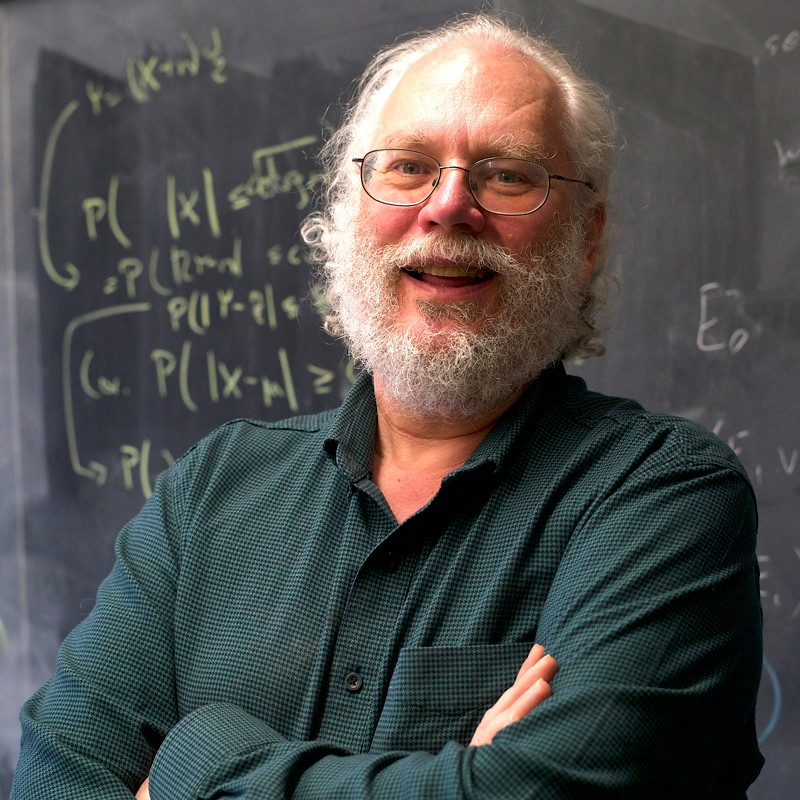
\includegraphics[height=3.5cm,keepaspectratio]{images/peter-shor.jpg}
        \end{center}
        
        It was developed in 1994 by the American mathematician Peter Shor.
    \end{frame}

    \begin{frame}{Classical part}
        \begin{alertblock}{Algorithm}
            \begin{enumerate}
                \item $a \overset{\$}{\leftarrow} [1, N-1]$
                \item Compute $K = gcd(N,a)$
                \item \textbf{if} $K \neq 0 $ ($\implies K$ is nontrivial factor of $N$) \textbf{then}
                \item \hspace{0.5cm} $r \leftarrow \text{quantum-period-finding-subroutine}(N,a)$
                \item \hspace{0.5cm} \textbf{if} ($r$ is odd $\; || \; a^{r/2} \equiv -1 \; mod \; N$)   \textbf{then} \\ \hspace{1cm} go to 1
                \item \hspace{0.5cm} \textbf{else} \\ \hspace{1cm} \textbf{return} $gcd(a^{r/2} + 1, N), gcd(a^{r/2} - 1, N)$
                \item \textbf{else} go to $1$
            \end{enumerate}
        \end{alertblock}

        Where the gcd function is computed using the Euclidean Algorithm.
    \end{frame}

    \begin{frame}{Quantum part: period-finding subroutine}
        The main idea is to use the quantum phase estimation on the unitay
        operator $$ U|y \rangle \equiv ay \; mod \; N \rangle$$

        \begin{exampleblock}{Example}
            With $a = 7$ and $N = 15$
            \begin{align*}
                U|1 \rangle &= |7 \rangle \\
                U^2|1 \rangle &= |4 \rangle \\
                U^3|1 \rangle &= |13 \rangle \\
                U^4|1 \rangle &= |1 \rangle
            \end{align*}
        \end{exampleblock}
    \end{frame}

    \begin{frame}{Example}
        \centering
        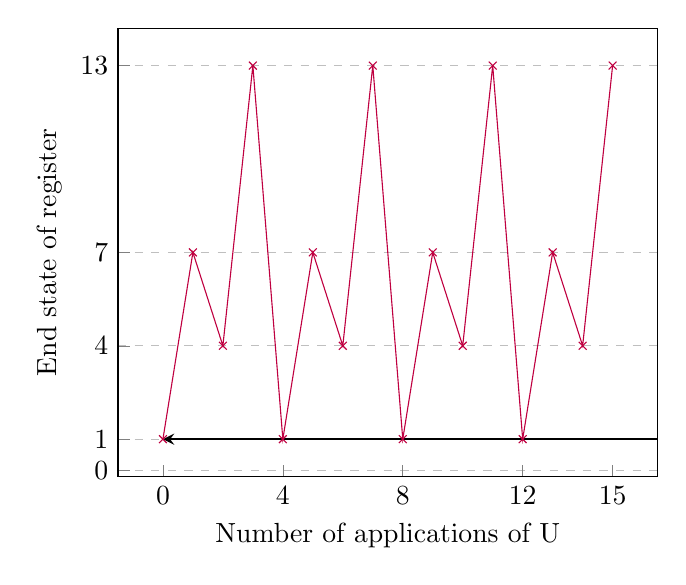
\begin{tikzpicture}
            \begin{axis}[
                xlabel={Number of applications of U},
                ylabel={End state of register},
                xtick={0,4,8,12,15},
                ytick={0, 1, 4, 7, 13},
                ytick pos= left,
                xtick pos= left,
                ymajorgrids=true,
                grid style=dashed,
            ]

            \addplot[
                color=purple,
                mark=x,
            ]
            coordinates {
                (0,1)(1,7)(2,4)(3,13)(4,1)(5,7)(6,4)(7,13)(8,1)(9,7)(10,4)(11,13)(12,1)(13,7)(14,4)(15,13)
            };

            \draw[stealth-stealth, thick](0,1) -- (40,1) node[midway,above]{\small $r$};


            \end{axis}
        \end{tikzpicture}
    \end{frame}

    \begin{frame}{}
    \end{frame}

    \section{Implementation}
    
    
\end{document}
